\chapter{常见曲面}
“本章中,我们要讨论一类特殊的拓扑空间:闭曲面,它是拓扑学(特别是代数拓扑学和低维拓扑学)中最重要的研究对象之一,也常在许多别的数学分支中出现.我们将讨论闭曲面的拓扑分类问题.
商空间概念给出了一种从已有拓扑空间构造新空间的方法.这种方法在代数拓扑学中是很有用的.它也将是本章研究闭曲面时所用的主要方法.”

\section{几个常见曲面}
在曲面中,除了平面\(E^2\)和球面\(S^2\)外,常见的是平环,Mobius带,环面,Klein瓶和射影平面.它们都可以用矩形面块经过粘合而得到
\subsection*{平环和Mobius环}
把矩形面块弯曲并将两侧边粘结,得到一个截圆柱面(图\ref{fig:enter-label})
\begin{figure}[H]
    \centering
    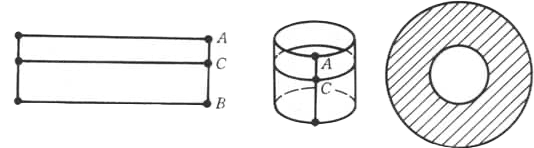
\includegraphics[width=0.5\linewidth]{image.png}
    \caption{平环}
    \label{fig:enter-label}
\end{figure}
“它同胚于平面上由两个同心圆所夹的环带,因此拓扑上称它为平环.确切地说,平环是一个拓扑等价类中诸空间的统称,不论这个空间确实是一环带,还是圆柱面或其他形状,也不管它的大小,只要属于该拓扑等价类,都称作平环.
制造平环时,只要将矩形弯曲而不要拧转,因此矩形两侧边上同高度的点相粘合.图3-1中,矩形两侧标相同文字的点表示要粘合在一起的.如果先将矩形拧转180°,再将两侧边粘接(如图\ref{fig:enter-label_2}),所得空间就是著名的Möbius带.”
\begin{figure}[H]
    \centering
    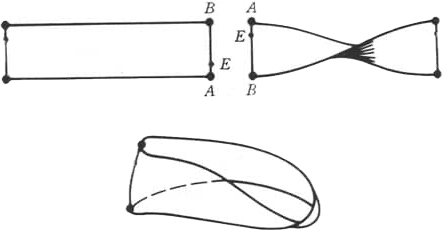
\includegraphics[width=0.5\linewidth]{image_2.png}
    \caption{Mobius带}
    \label{fig:enter-label_2}
\end{figure}
\subsection*{环面和Klein瓶}
“环面和Klein瓶都可以用一截圆柱面(平环)将两个截口互相粘接而得到.”
\begin{figure}[H]
    \centering
    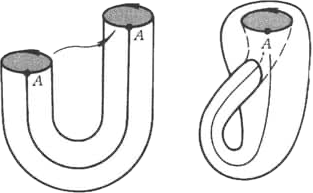
\includegraphics[width=0.5\linewidth]{image_3.png}
    \caption{环面}
    \label{fig:enter-label_3}
\end{figure}
“如果每一直母线段的两端粘合,所得到的是环面(图\ref{fig:enter-label_3}),两个截口是以相同的方向相粘接的.如果让两个截口方向相反地粘接,则得到Klein瓶(图\ref{fig:enter-label_4}).要实现这样的粘接,必须将圆柱面弯曲后,把一端穿过管壁进入管内与另一端相接.在3维空间中这是做不到的,因为在进入管内之处必然要相交.但在4维空间中可以实现(让相交点的第四个坐标不同,从而把它们分开).”
\begin{figure}[H]
    \centering
    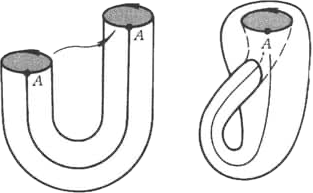
\includegraphics[width=0.5\linewidth]{image_3.png}
    \caption{Klein瓶}
    \label{fig:enter-label_4}
\end{figure}
“Klein瓶也是单侧的(图\ref{fig:enter-label_4}),以后要证明它与环面不同胚.环面是一种常见曲面.各种轮胎的表面是环面;圆周绕着与它共面但相离的轴线旋转得到环面(图\ref{fig:enter-label_5}),称此圆周上的点旋出的圆为纬圆,以轴线为界的半平面与环面的交线称为经圆;\(S^1 \times S^1\)是环面.一般地记\(T^n =S^1 \times S^1 \times S^1 \times \dots \times S^1\),称为n维环面.这里讨论的是2维环面\(T^2\).”
\begin{figure}[H]
    \centering
    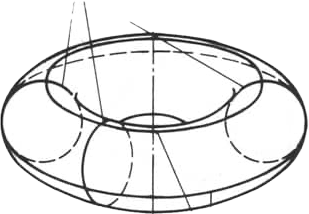
\includegraphics[width=0.5\linewidth]{image_5.png}
    \caption{环面}
    \label{fig:enter-label_5}
\end{figure}
和平环一样,环面和其他曲面都是一个拓扑等价类中空间的统称
\subsection*{射影平面}
“射影平面记作\(P^2\),它是射影几何学中的概念.拓扑学中,有几种描述它的方法,其中之一是把圆盘\(D^2\)(它同胚于矩形面块)的边界\(S^1\)上每一对对径点(同一直径的两个端点)粘合,得到射影平面(图\ref{fig:enter-label_6}).这种粘接直观上就不好理解了,在3维欧氏空间中是做不到的,在4维空间中能实现,但也不好想象.我们将在后面说清楚它.”
\begin{figure}[H]
    \centering
    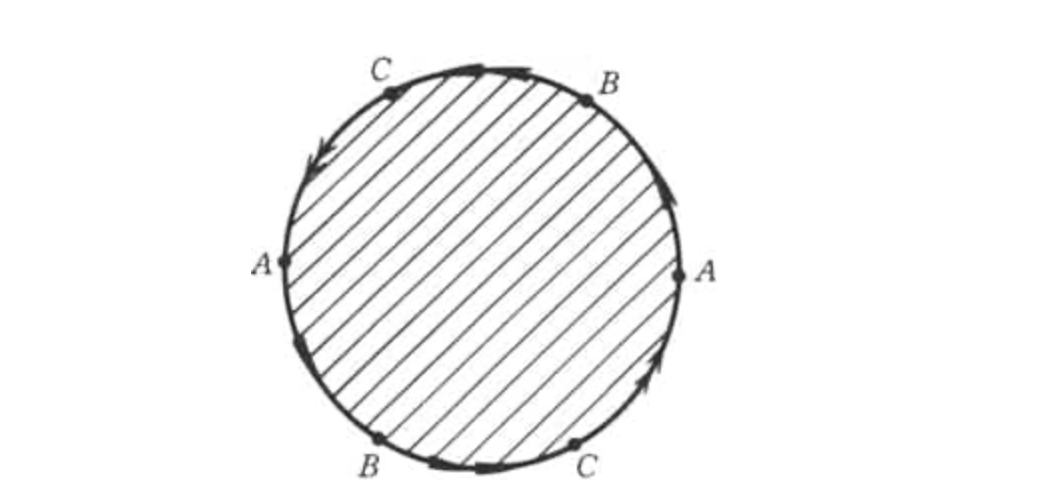
\includegraphics[width=0.5\linewidth]{image_6.png}
    \caption{射影平面}
    \label{fig:enter-label_6}
\end{figure}
“用“粘合”方法制造新拓扑空间是拓扑学中常用的一种方法.还有许多更复杂的“粘合”,凭直观是不好接受的.例如,把圆盘\(D^2\)与I的乘积空间\(D^2 \times I \)的一端(子集\(D^2 \times \left\{1\right\}\))捏为一点,得到的空间的直观形象是一个圆锥体(图\ref{fig:enter-label_7}).如果用一般拓扑空间X代替\(D^2\),得到的空间是什么?又如把环面上的一个经圆和一个纬圆捏在一起成一个点,又会得到什么空间?这些问题都不能靠直观来回答.”
\begin{figure}[H]
    \centering
    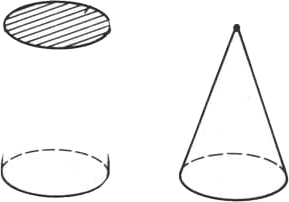
\includegraphics[width=0.5\linewidth]{image_7.png}
    \caption{}
    \label{fig:enter-label_7}
\end{figure}
\section{商空间与商映射}
\subsection*{商空间}
设拓扑空间X上作某种粘合得到新空间,如果把要粘在一起的点称为互相等价的点,X上就有了一个等价关系,每个等价类被粘合为新空间上的一个点,因此新空间的集合就是等价类的集合.一般地,一个集合X上如果有等价关系\(\sim\),相应的等价类的集合记作\(X / \sim \),称为X关于\(\sim \)的商集,把X上的点对应到它所在的等价类,得到映射\(p : X \rightarrow X / \sim\),称为粘合映射,设X已有了拓扑,现在我们来规定\(S / \sim \)上的一个拓扑.
\begin{definition}
    设\( X, \tau \)是拓扑空间,\(\sim\)是集合X上的一个等价关系,规定商集\(X / \sim \)上的子集族 
    \[\widetilde{\tau} := \left\{V \subset X / \sim | p^{-1}(V) \in \tau \right\}\]
    则\(\widetilde{\tau}\)是\(X / \sim \)上的一个拓扑,称为\(\tau\)在\(\sim\)下的商拓扑,称\((X /\sim , \widetilde{\tau} )  \)是\((X,\tau)\)关于\(\sim\)的商空间.简记为\(X / \sim\)
\end{definition}
按照定义,\(X / \sim \)的开集也就是在p之下的原像是X中开集的那些子集,显然\(p : X \rightarrow X / \sim \)是连续的;并且,如果集合\(X / \sim \)上另有拓扑\(\tau^{'}\)使得p连续,则 \(\tau^{'} \subset \widetilde{\tau}\),因此\(\widetilde{\tau}\)是\(X / \sim\)上使得粘合映射p连续的最大的拓扑 . 
\begin{theorem}
    设X,Y是两个拓扑空间,\(\sim\)是X上的一个等价关系,\(g: X/\sim \rightarrow Y \)是一映射,则g连续\(\Leftrightarrow\)\(g*p\)连续
    \end{theorem}
    下面利用商空间概念规定一种常见的空间:
\\
设A是拓扑空间X的一个子集(通常是闭子集),把A捏为一点(也就是将A看作一个等价类,别的点各自成一个等价类),得到的商空间记作\(X / A \) \\
对于任一的拓扑空间X记 \[C_x := X \times I / X \times \left\{1\right\}\] 称为X的拓扑锥 \\
如果\(X \subset E^n\),取\(a \in E^{n+1} / E^n\),规定\(E^{n+1}\)的子集: 
\[a_X := \left\{ta +(1-t)a \right\}\]
称为X上以a为顶点的几何锥,同时如果X是\(E^n\)的紧致子集,则\(a_X \cong C_X \)
 \subsection*{商映射}
 商映射和商空间是紧密相关的概念,可以说它们是从不同的角度看同一事物,商映射是从映射的角度观察,更有利于加深认识.
\begin{definition}
    设X和Y是拓扑空间,映射\(f : X \rightarrow Y \)称为商映射,如果
    \begin{enumerate}
        \item f是连续映射; \\
        \item f 是满的 ;\\
        \item 设\(B \subset Y \),如果\(f^{-1}(B)\)是X的开集,则B是Y的开集.
    \end{enumerate}
\end{definition}
\begin{theorem}
    若\(f: X \rightarrow X^{'}\)是商映射,\(g: X^{'} \rightarrow Y\)是一映射,则g连续\(\Leftrightarrow\) \(g*f\)连续 .
\end{theorem}
\begin{corollary}
    如果\(f: X \rightarrow Y\)是商映射,则\(X / \overset{f}{\sim} \cong Y \)  
\end{corollary}
\begin{corollary}
    连续的满映射\(f : X \rightarrow Y  \) 如果还是开映射或闭映射,则它是商映射
\end{corollary}
\begin{example}
    乘积空间\(X \times Y \)到X的投射j是满的连续开映射,从而它是闭映射
\end{example}
下面是一个实用价值很大的判定上商映射的充分条件
\begin{theorem}
    如果X紧致,Y是Hausdorff 空间,则连续满映射\(f: X \rightarrow Y \)一定是商映射
\end{theorem}
从定义可以看出:单一的商映射就是同胚.
\begin{corollary}
    商映射的复合也是商映射
\end{corollary}
\subsection*{射影平面的定义形式}
先回顾在第一节中提到的定义:把圆盘\(D^2\)(它同胚于矩形面块)的边界\(S^1\)上每一对对径点(同一直径的两个端点)粘合,得到射影平面(图\ref{fig:enter-label_6}).
接着再给出其余的定义
:
\\
(1):作\(g: D^2 \rightarrow S^2\)为\(g(x,y) = (x,y,\sqrt{1-x^2-y^2}) \),则\(f*g : D^2 \rightarrow P^2\)也是商映射,因此\(D^2\)上粘合\(S^1\)的各对径点得到\(P^2\)(图\ref{fig:enter-label_8})
\begin{figure}[H]
    \centering
    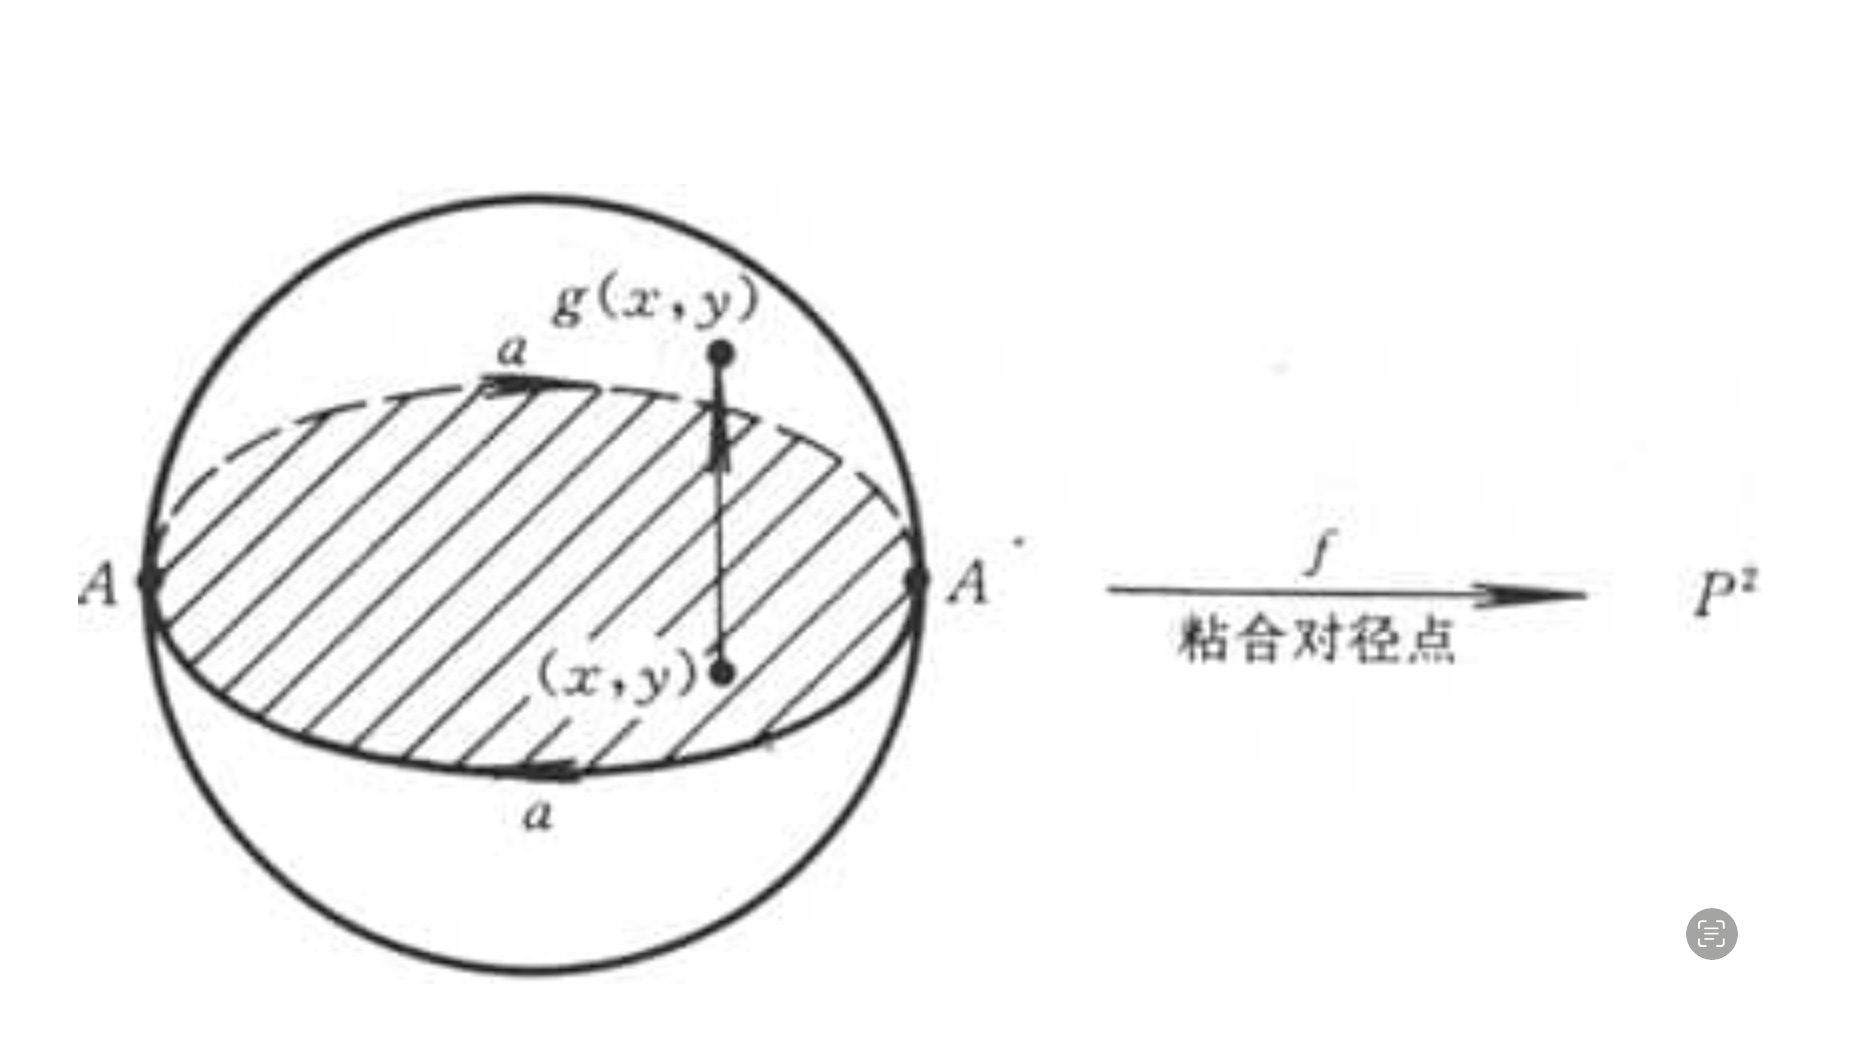
\includegraphics[width=0.5\linewidth]{image_8.png}
    \caption{}
    \label{fig:enter-label_8}
\end{figure}
(2):沿边界,将Mobius带和\(D^2\)粘合在一起,商空间就是\(P^2\) (图\ref{fig:enter-label_9})
\begin{figure}[H]
    \centering
    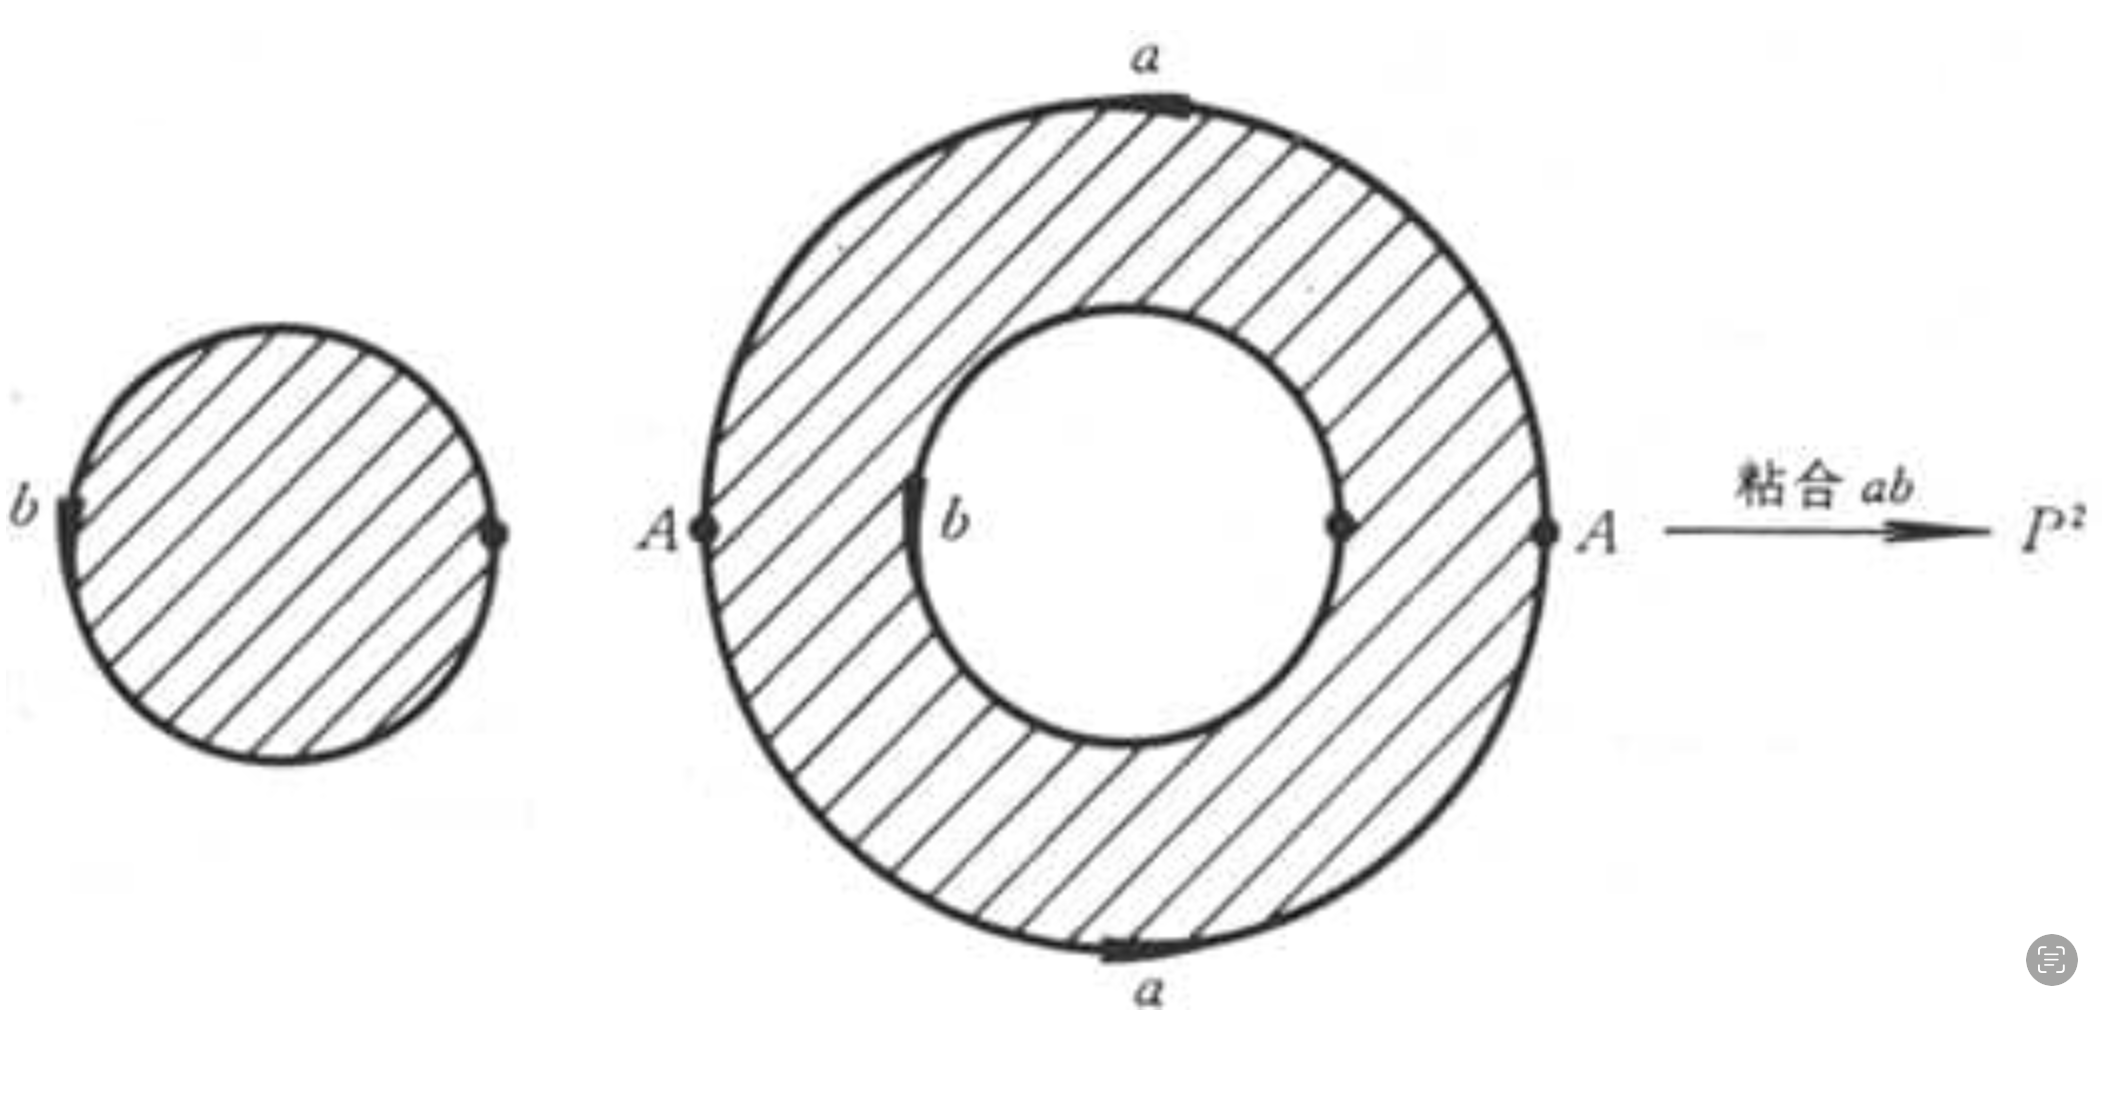
\includegraphics[width=0.5\linewidth]{image_9.png}
    \caption{}
    \label{fig:enter-label_9}
\end{figure}
\subsection*{关于商映射的定理}
设\(f_i : X_i \rightarrow Y_i,\quad (i =1 ,2)\)是映射,规定映射
\[f_1 \times f_2 : X_1\times X_2 \rightarrow Y_1 \times Y_2\]
为\((f_1 \times f_2 ) (x_1,X_2) = (f_1(x) ,f_2(x))\).显然,当\(f_1 ,f_2\)都为满映射时\(f_1 \times f_2 \)也是满映射,当\(f_1\)和\(f_2\)都是连续映射时\(f_1 \times f_2\) 也是连续映射 .
\begin{theorem}
    设\(f: X \rightarrow Y \)是商映射,Z是局部紧致的Hausdorff 空间,\(id : Z \rightarrow Z \)表示恒同映射,则
    \[f \times id ; X \times Z \rightarrow Y \times Z\]
    也是商映射
\end{theorem}
\begin{theorem}
    设A是Hausdorff空间X的紧致子集,则\(X /A \)也是 Hausdorff空间 .
\end{theorem}
\begin{theorem}
    设M是Mobius 带,\(\partial M \)是它的边界,则\(M / \partial M \cong P^2\)
\end{theorem}
\section{拓扑流形与闭曲面}
\subsection*{流形}
“球面、环面以及我们熟悉的其他曲面从整体上看比平面复杂多了,但是在局部上,它们每一点的近旁都有一块区域同胚于平面.这种特性使得我们可以在局部的范围内应用分析学工具对它进行研究.粗略地讲,具有局部欧氏特性的拓扑空间称之为流形.它是近代数学最重要的基础概念之一.它不仅在几何学科中占有重要地位,在分析学科和应用数学中也是重要研究对象.流形是比较复杂的概念,在不同的研究领域还要求它带有各种特殊的结构.下面定义的拓扑流形是最一般的流形.”
\begin{definition}
    一个Hausdorff空间X称为n维(拓扑)流形,如果X的任一点都有一个同胚于\(E^n\)或\(E^n_{+}\)的开邻域
\end{definition}
\begin{note}
    注明: 这里得\(E^n_{+}\)是半个n维欧氏空间,规定为: 
    \[E^n_{+} := \left\{(x_1,x_2 ,\dots ,x_n) \in E^n | x_n \geq 0\right\}\]
    按照这个定义,\(E^n ,D^n, S^n , T^n\) 均是n维流形 , 但是二次锥面不是流形,去除掉顶点的二次锥面才算是流形(因为二次锥面的顶点的任一邻域不同胚于\(E^n \text{或}E^n_{+}\)
\end{note}
从定义易知: 流形满足\(C_1\)公理,它还是局部道路连通和局部紧致的,同时n维流形有边界点,则记\(\partial M \)是它的边界点的集合且是一个(n-1) 维的流形 .
\subsection*{闭曲面}
二维流形称为曲面 . 
\begin{definition}
    没有边界点的紧致连通曲面称为闭曲面 . 
\end{definition}
\begin{theorem}
    一般地,假设 「是一个偶数边的多边形,如果成对地粘接「 的边,那么所得的商空间是闭曲面.
\end{theorem}
\subsection*{两类闭曲面}
球面是最简单的闭曲面,对球面使用手术,可以得到许多新的闭曲面.
\subsection*{安环柄的球面}
环面上挖去一个开圆盘,就说是在环面上挖一个洞,把所得空间称为环柄 (图\ref{fig:enter-label_10})
\begin{figure}[H]
    \centering
    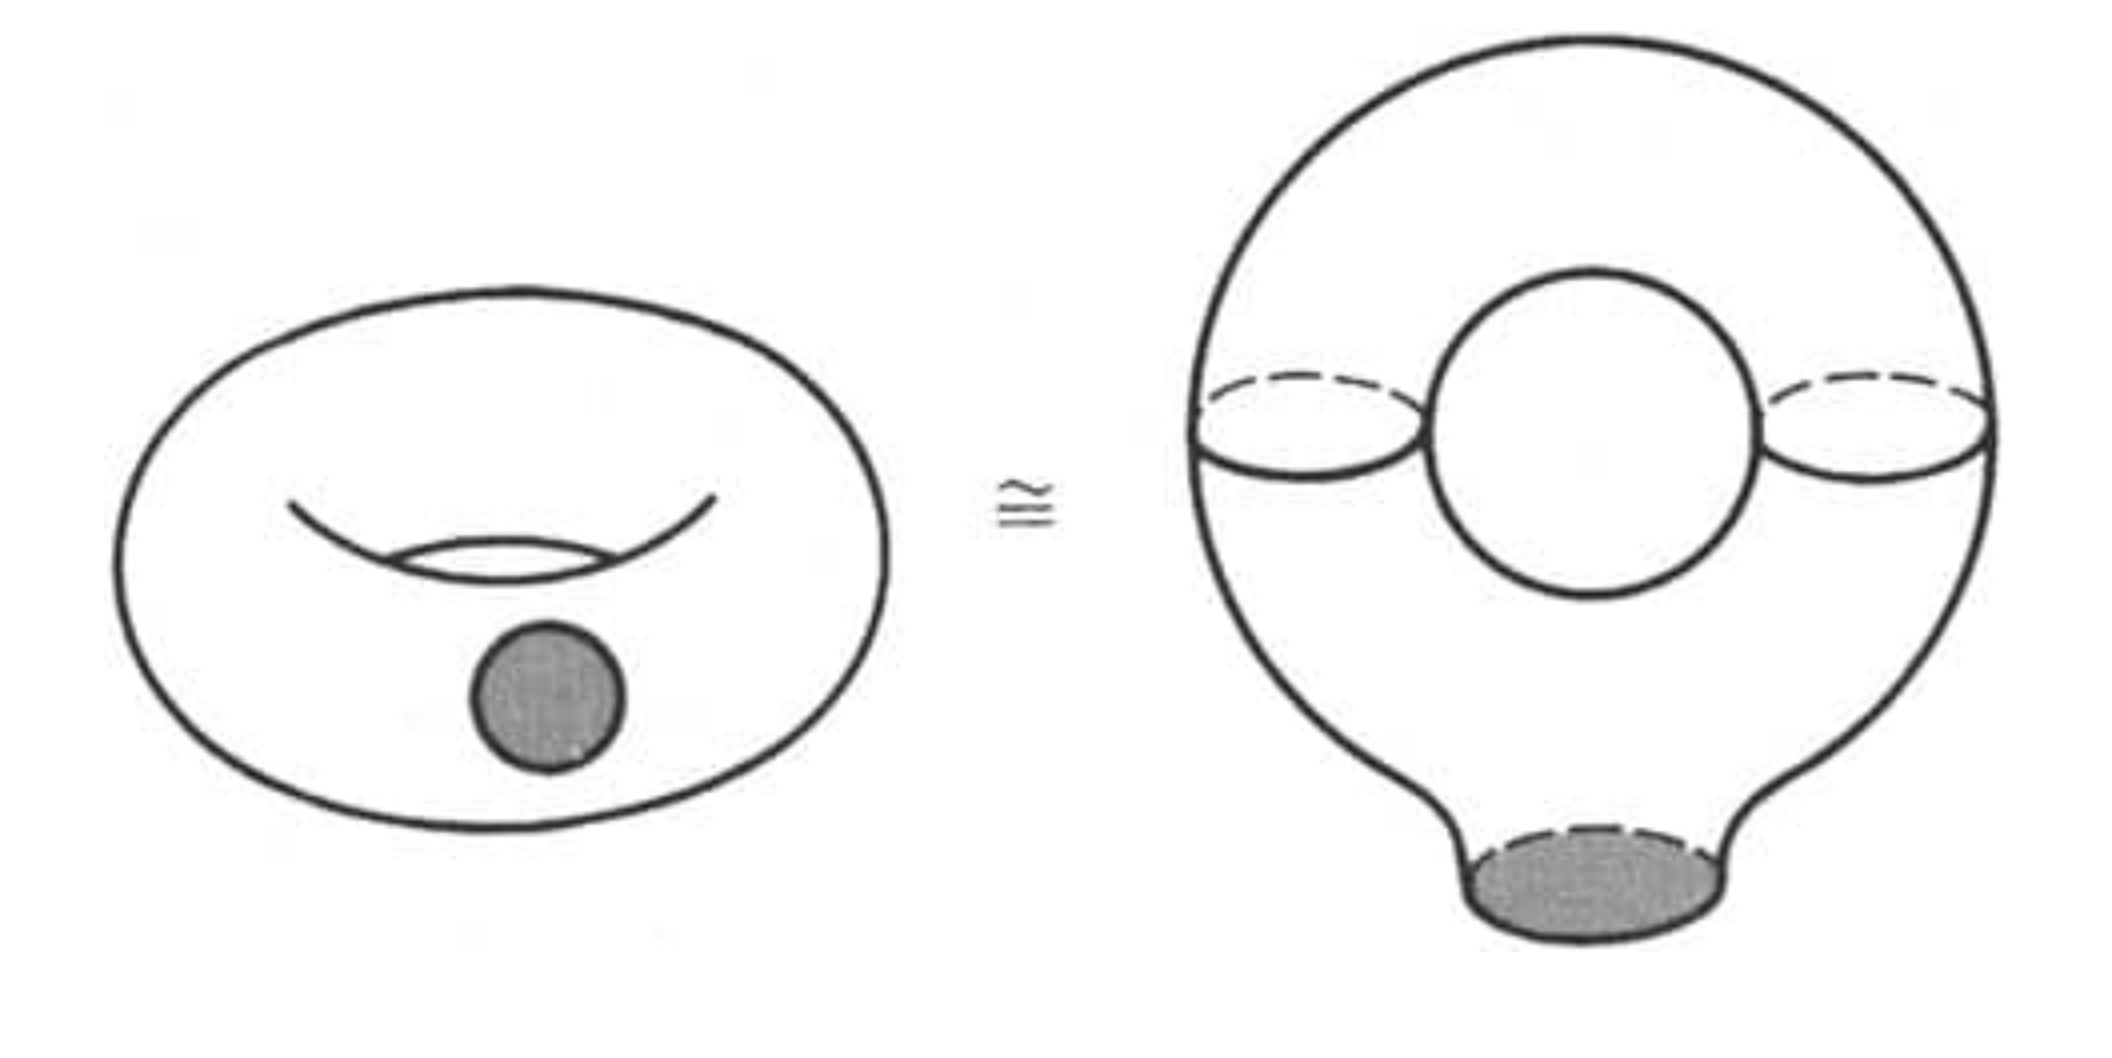
\includegraphics[width=0.5\linewidth]{image_10.png}
    \caption{}
    \label{fig:enter-label_10}
\end{figure}
在球面上挖一洞,在洞口粘接上一个环柄(图\ref{fig:enter-label_11})
\begin{figure}[H]
    \centering
    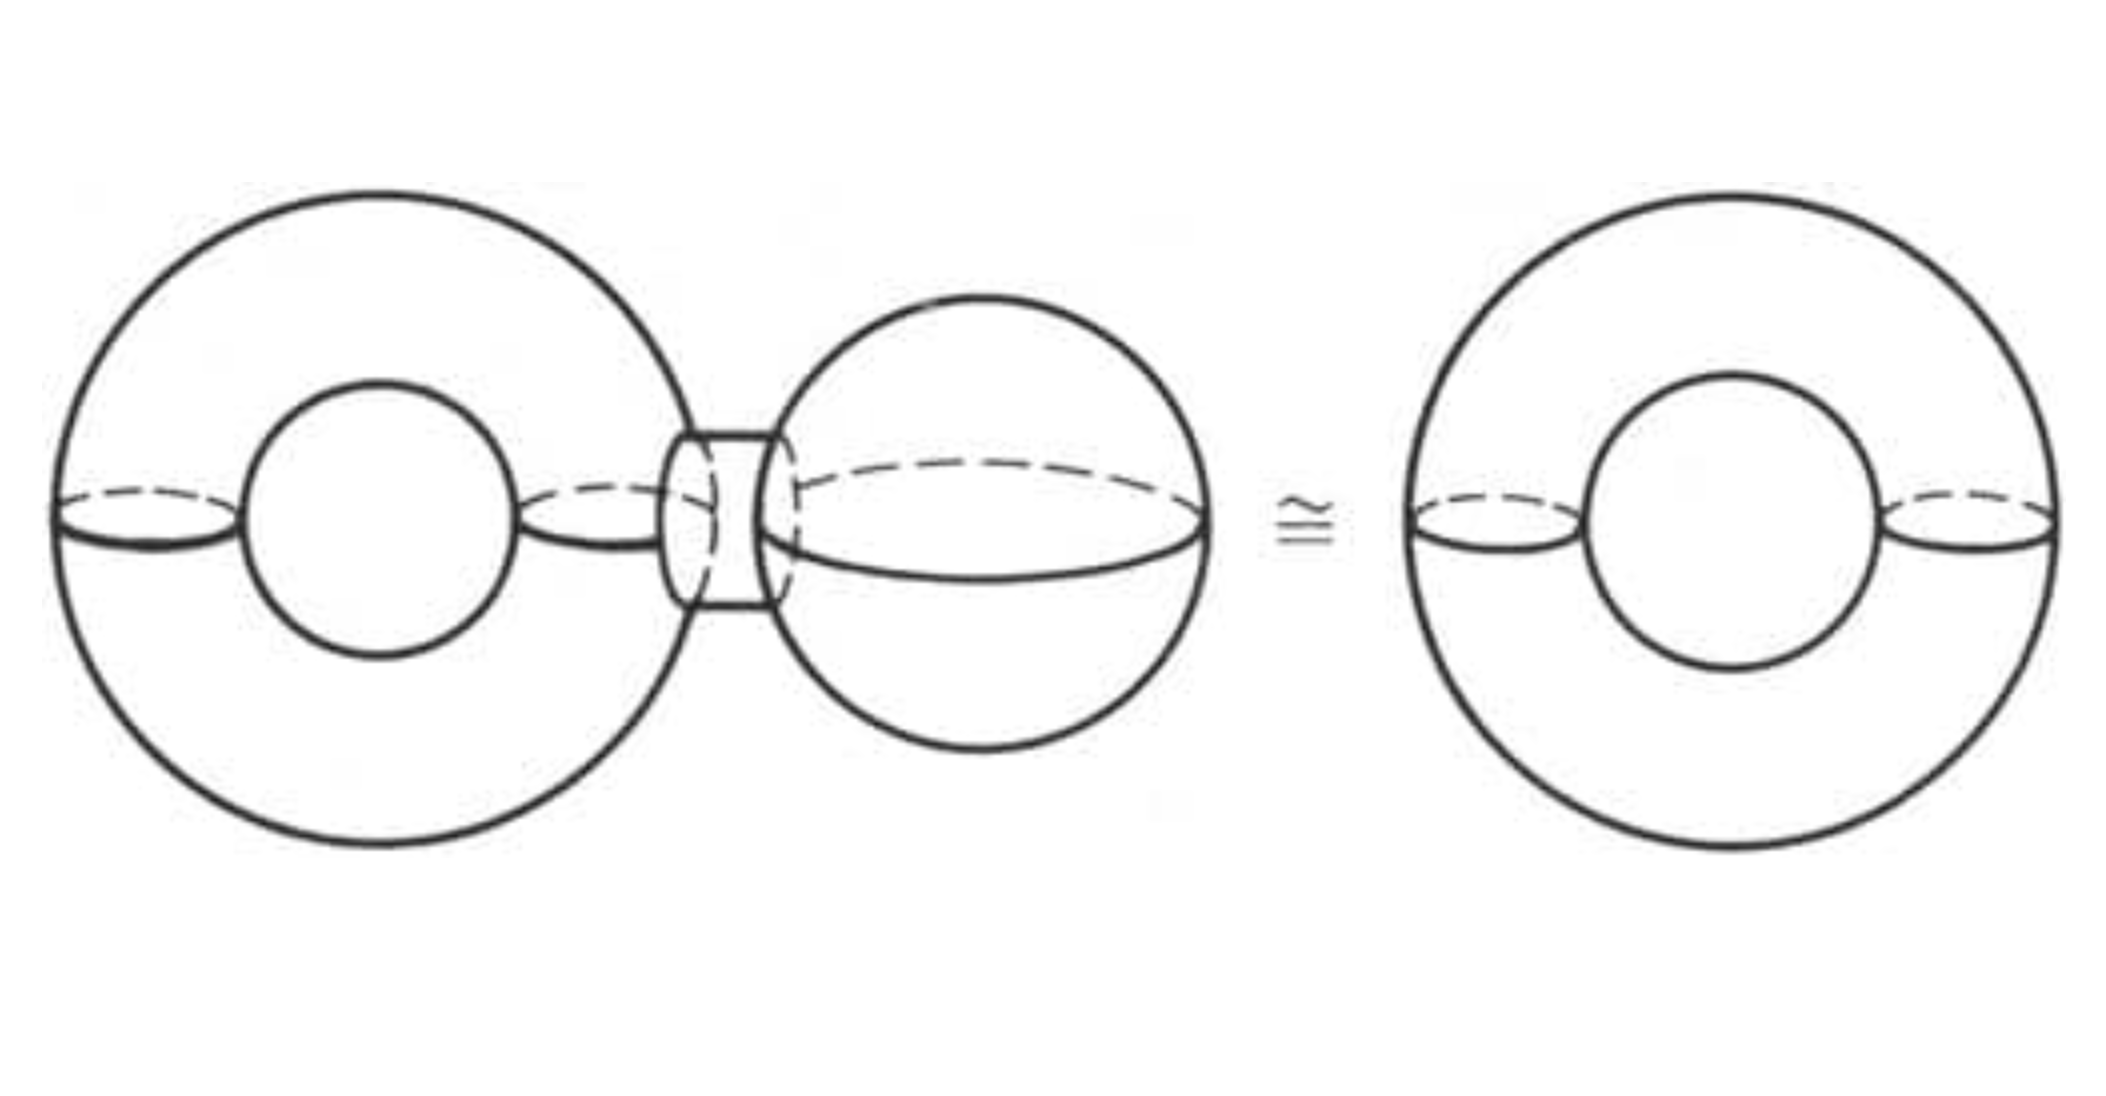
\includegraphics[width=0.5\linewidth]{image_11.png}
    \caption{}
    \label{fig:enter-label_11}
\end{figure}
把这样的“手术”称为在球面上安一个环柄.不难看出,得到的闭曲面是\(T^2\),如果在球面上安n个环柄,把得到的闭曲面记作\(nT^2\),称为亏格为n的可定向闭曲面. 由于安环柄时的洞口大小和位置(只要不相重叠)对所得闭曲面的拓扑类并不会影响,因此\(nT^2\)表示一个拓扑等价类.\(nT^2\)的另一种常用的形式就是n-环面(不同于n维环面)
\begin{figure}[H]
    \centering
    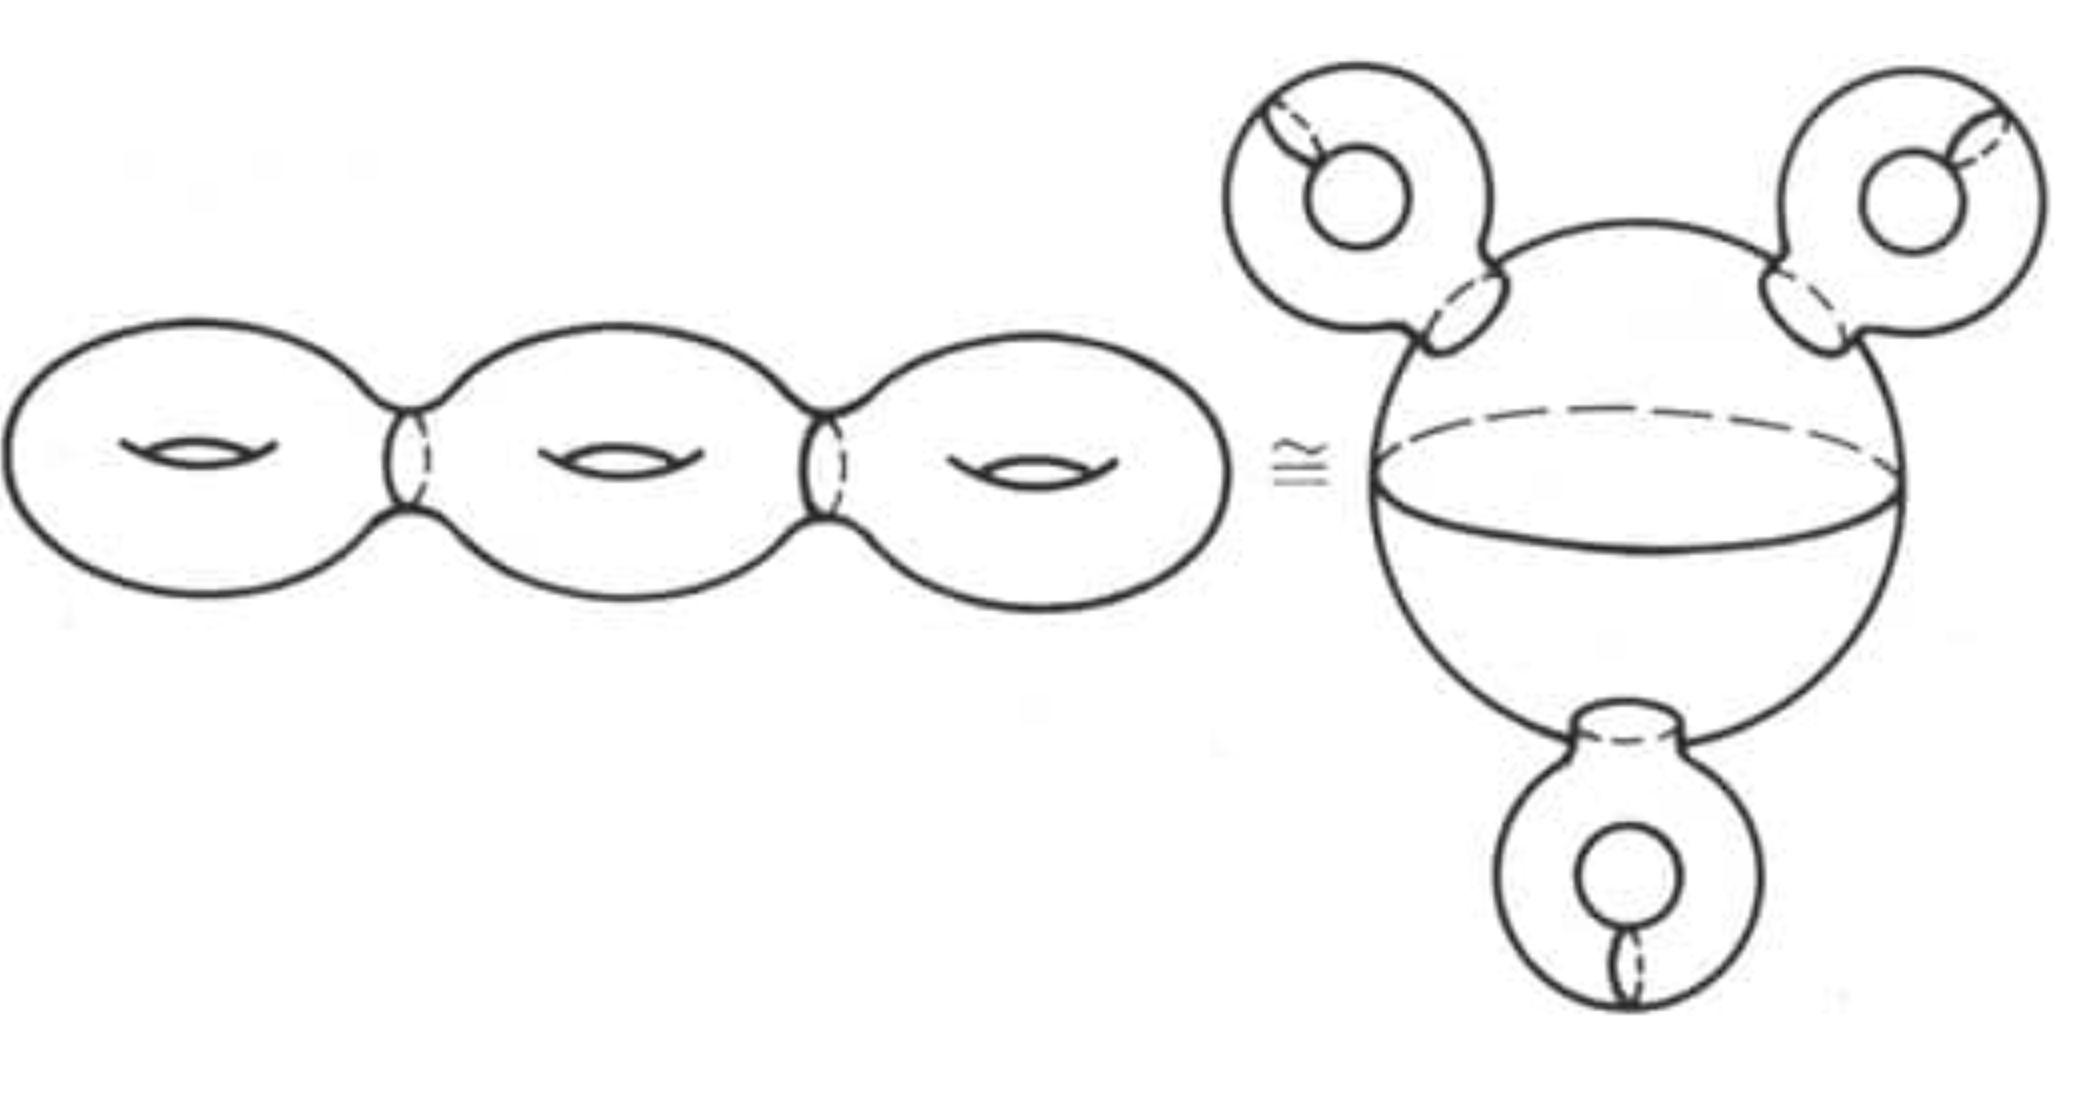
\includegraphics[width=0.5\linewidth]{image_12.png}
    \caption{}
    \label{fig:enter-label_!2}
\end{figure}
\subsection*{安交叉帽的球面}
“在球面上挖一洞,并在洞口粘接一条Möbius带,把这种手术称为在球面上安交叉帽.安了m个交叉帽的球面称为亏格为m的不可定向闭曲面,记作\(mP^2\)”
\begin{figure}[H]
    \centering
    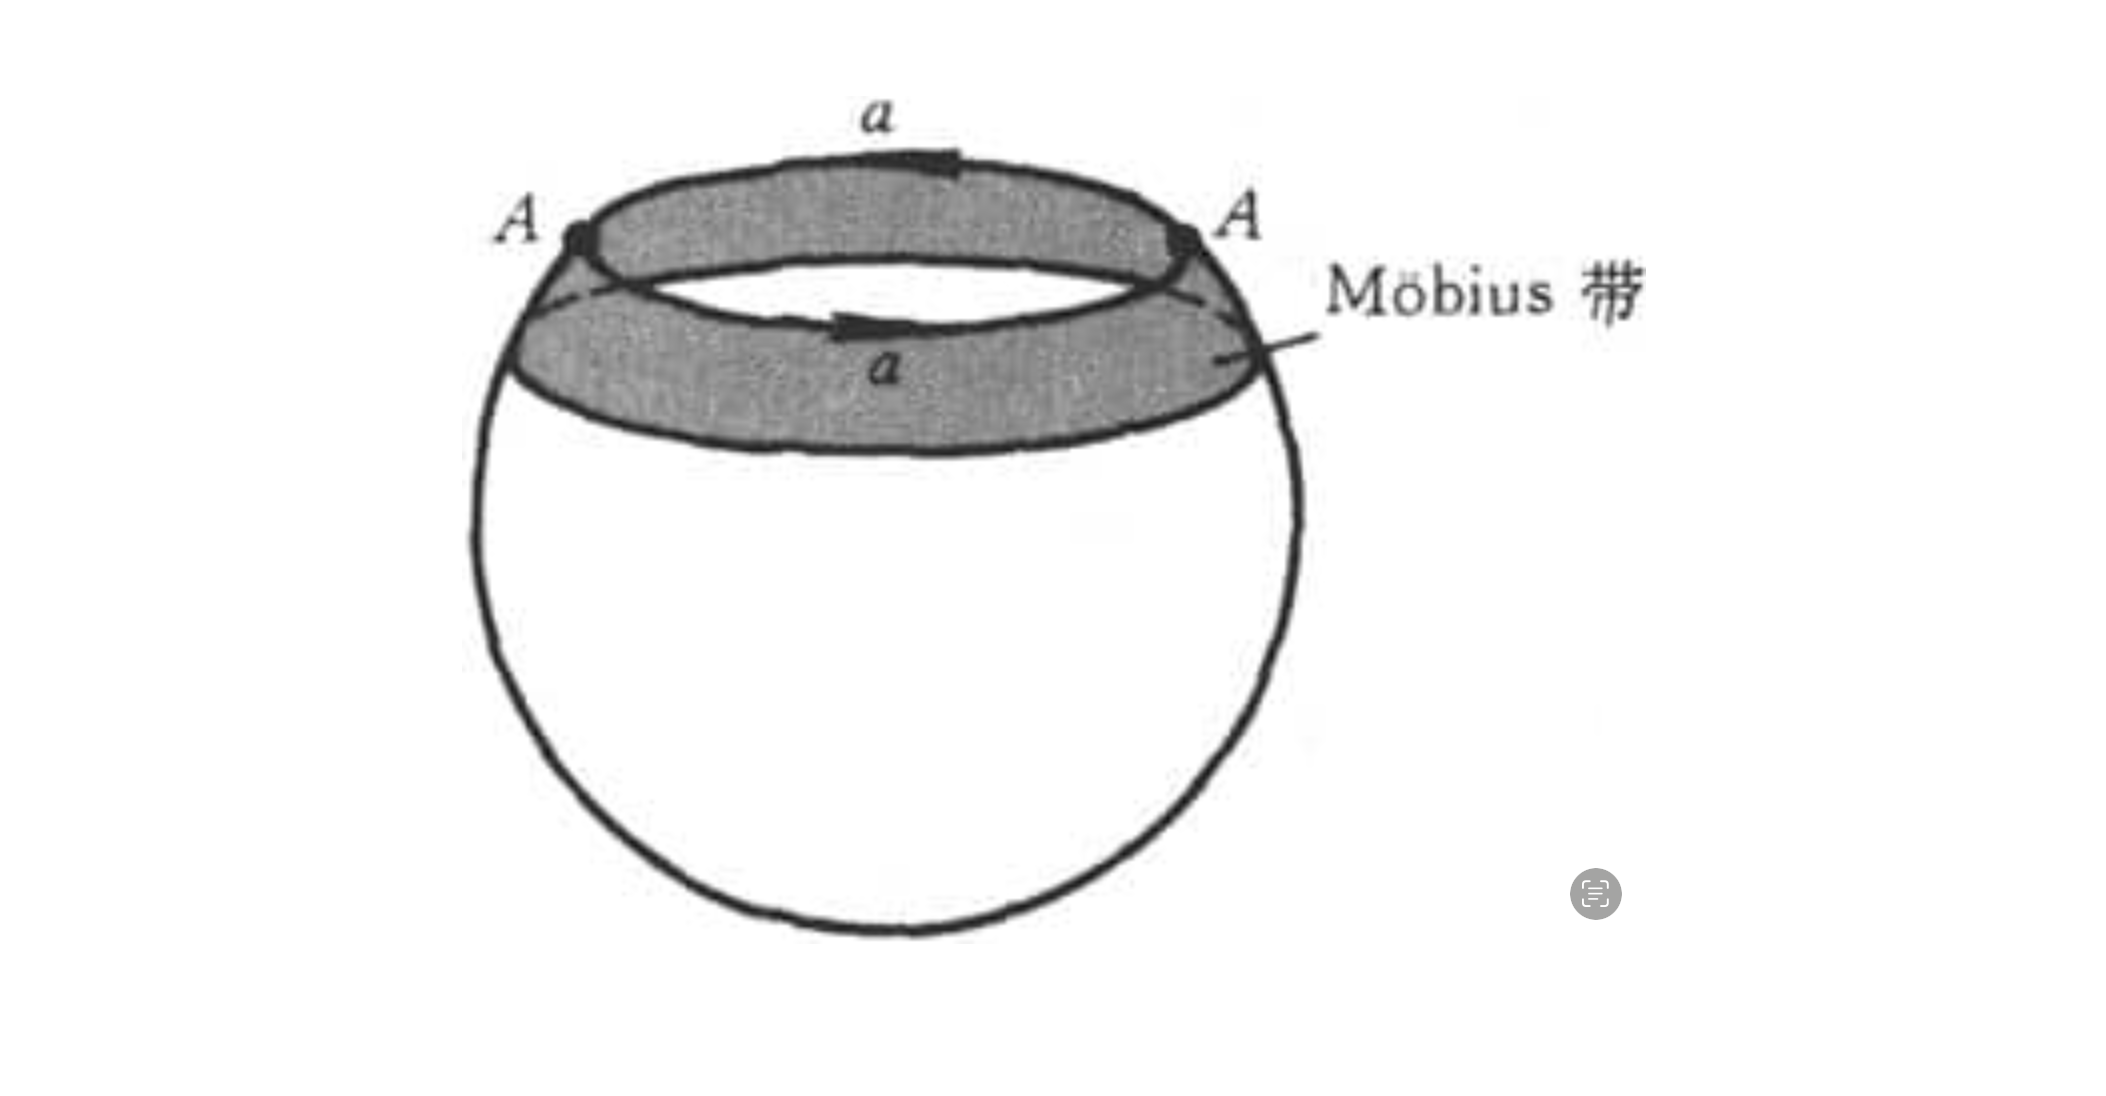
\includegraphics[width=0.5\linewidth]{image_13.png}
    \caption{}
    \label{fig:enter-label_13}
\end{figure}
安交叉帽的一种等效手术是将球面上洞口的对径点粘合.
\begin{figure}[H]
    \centering
    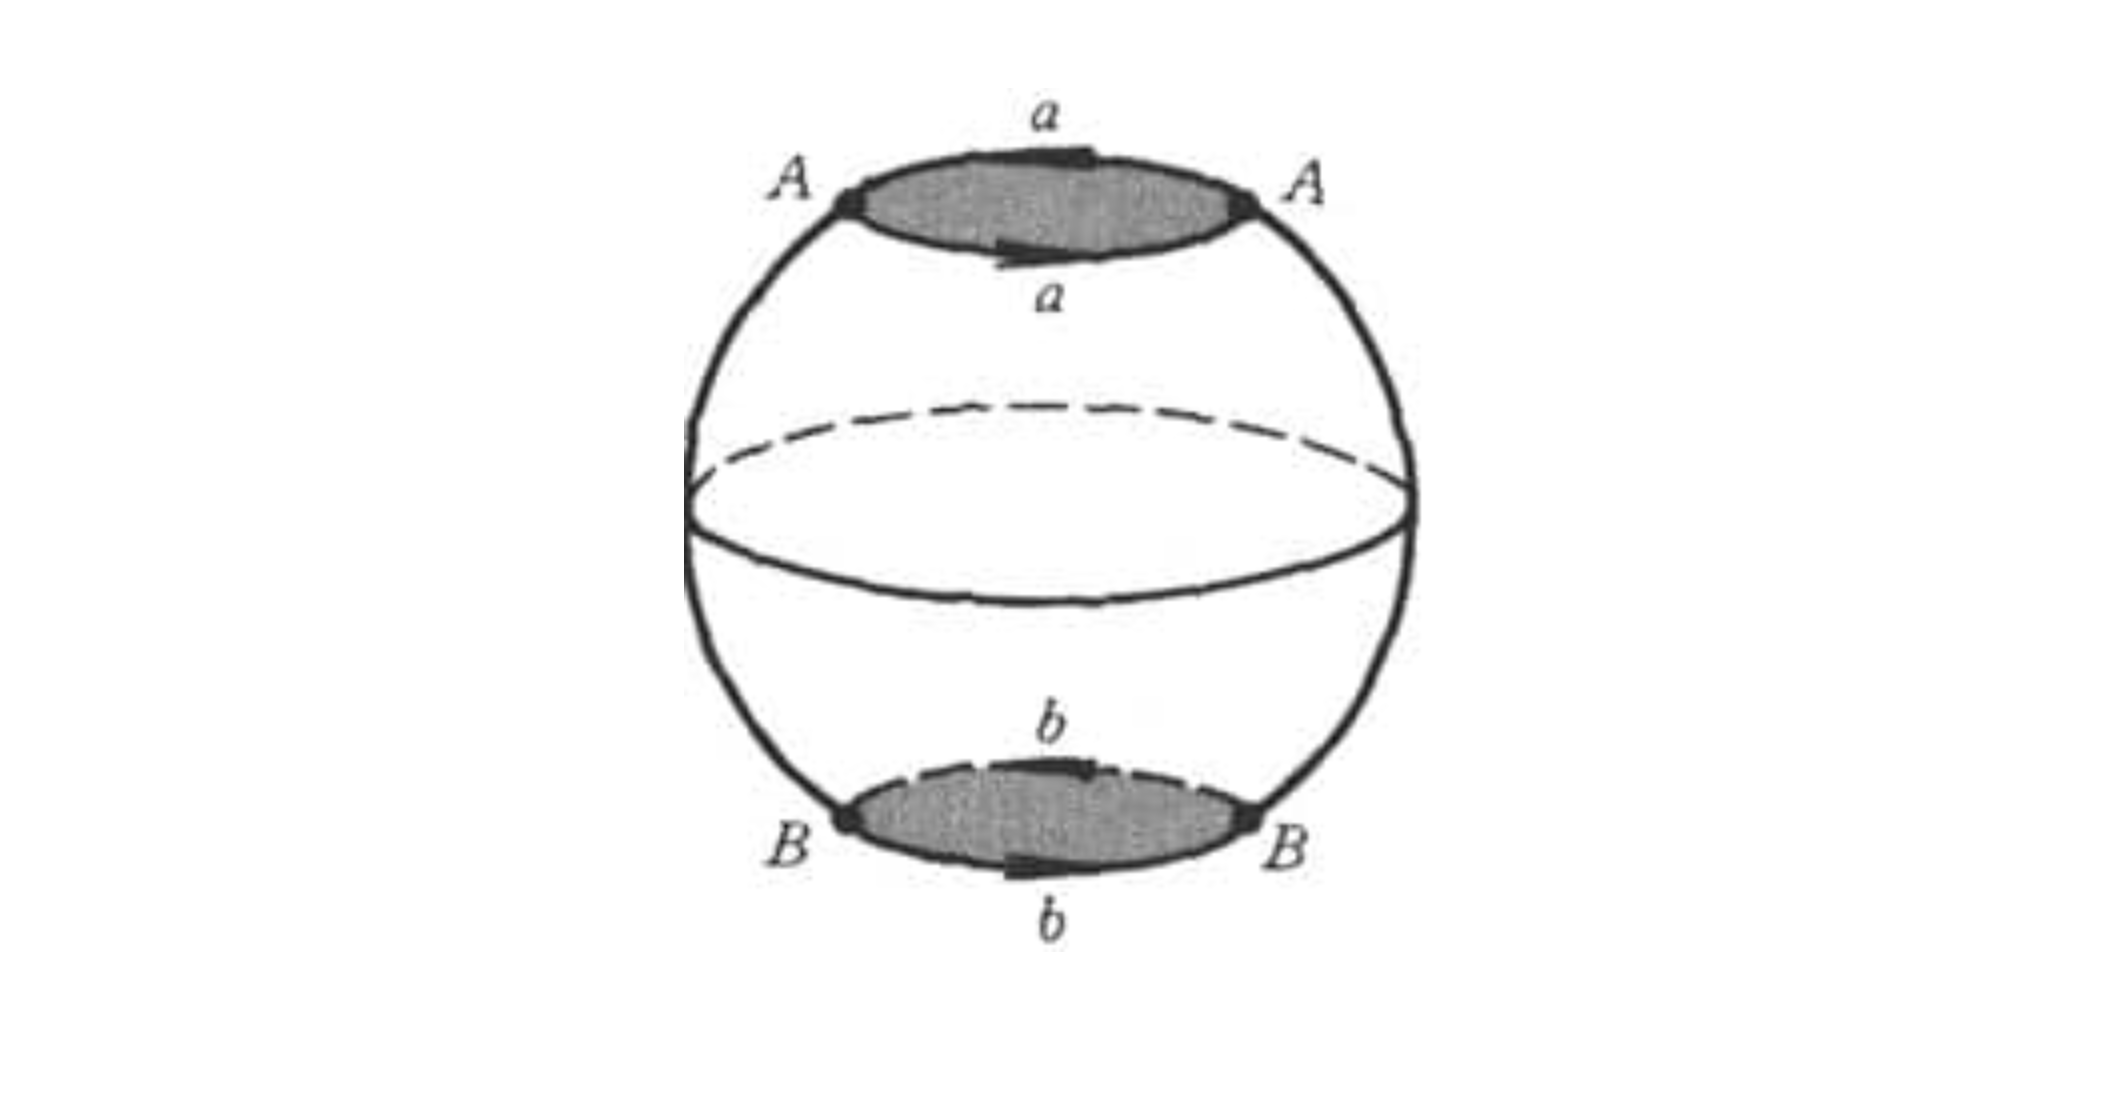
\includegraphics[width=0.5\linewidth]{image_14.png}
    \caption{}
    \label{fig:enter-label_14}
\end{figure}

\subsection*{一些粘合流程图}
将三角形两边粘接
\begin{figure}[H]
    \centering
    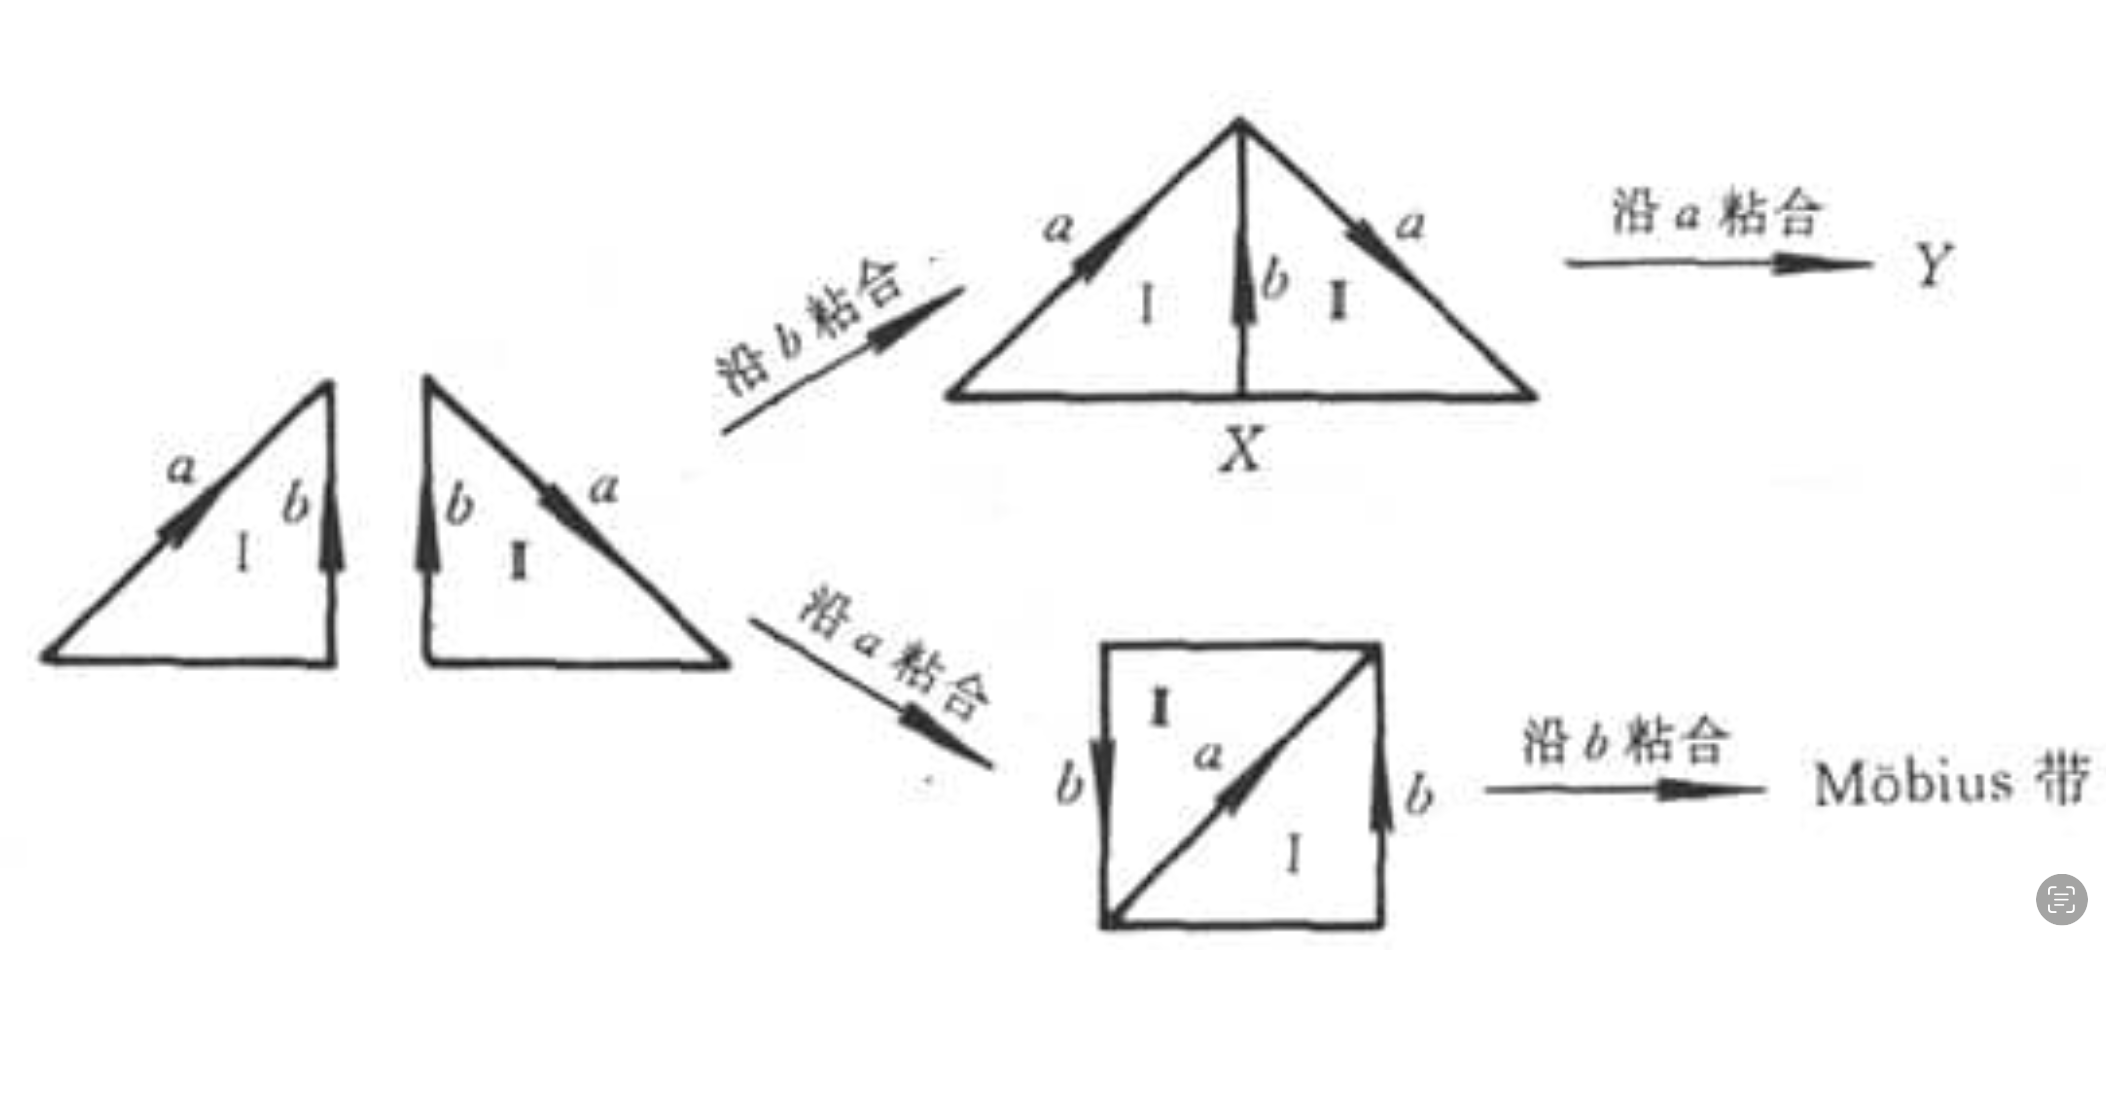
\includegraphics[width=0.5\linewidth]{image_15.png}
    \caption{}
    \label{fig:enter-label_15}
\end{figure}
“矩形的两对邻边粘接”
\begin{figure}[H]
    \centering
    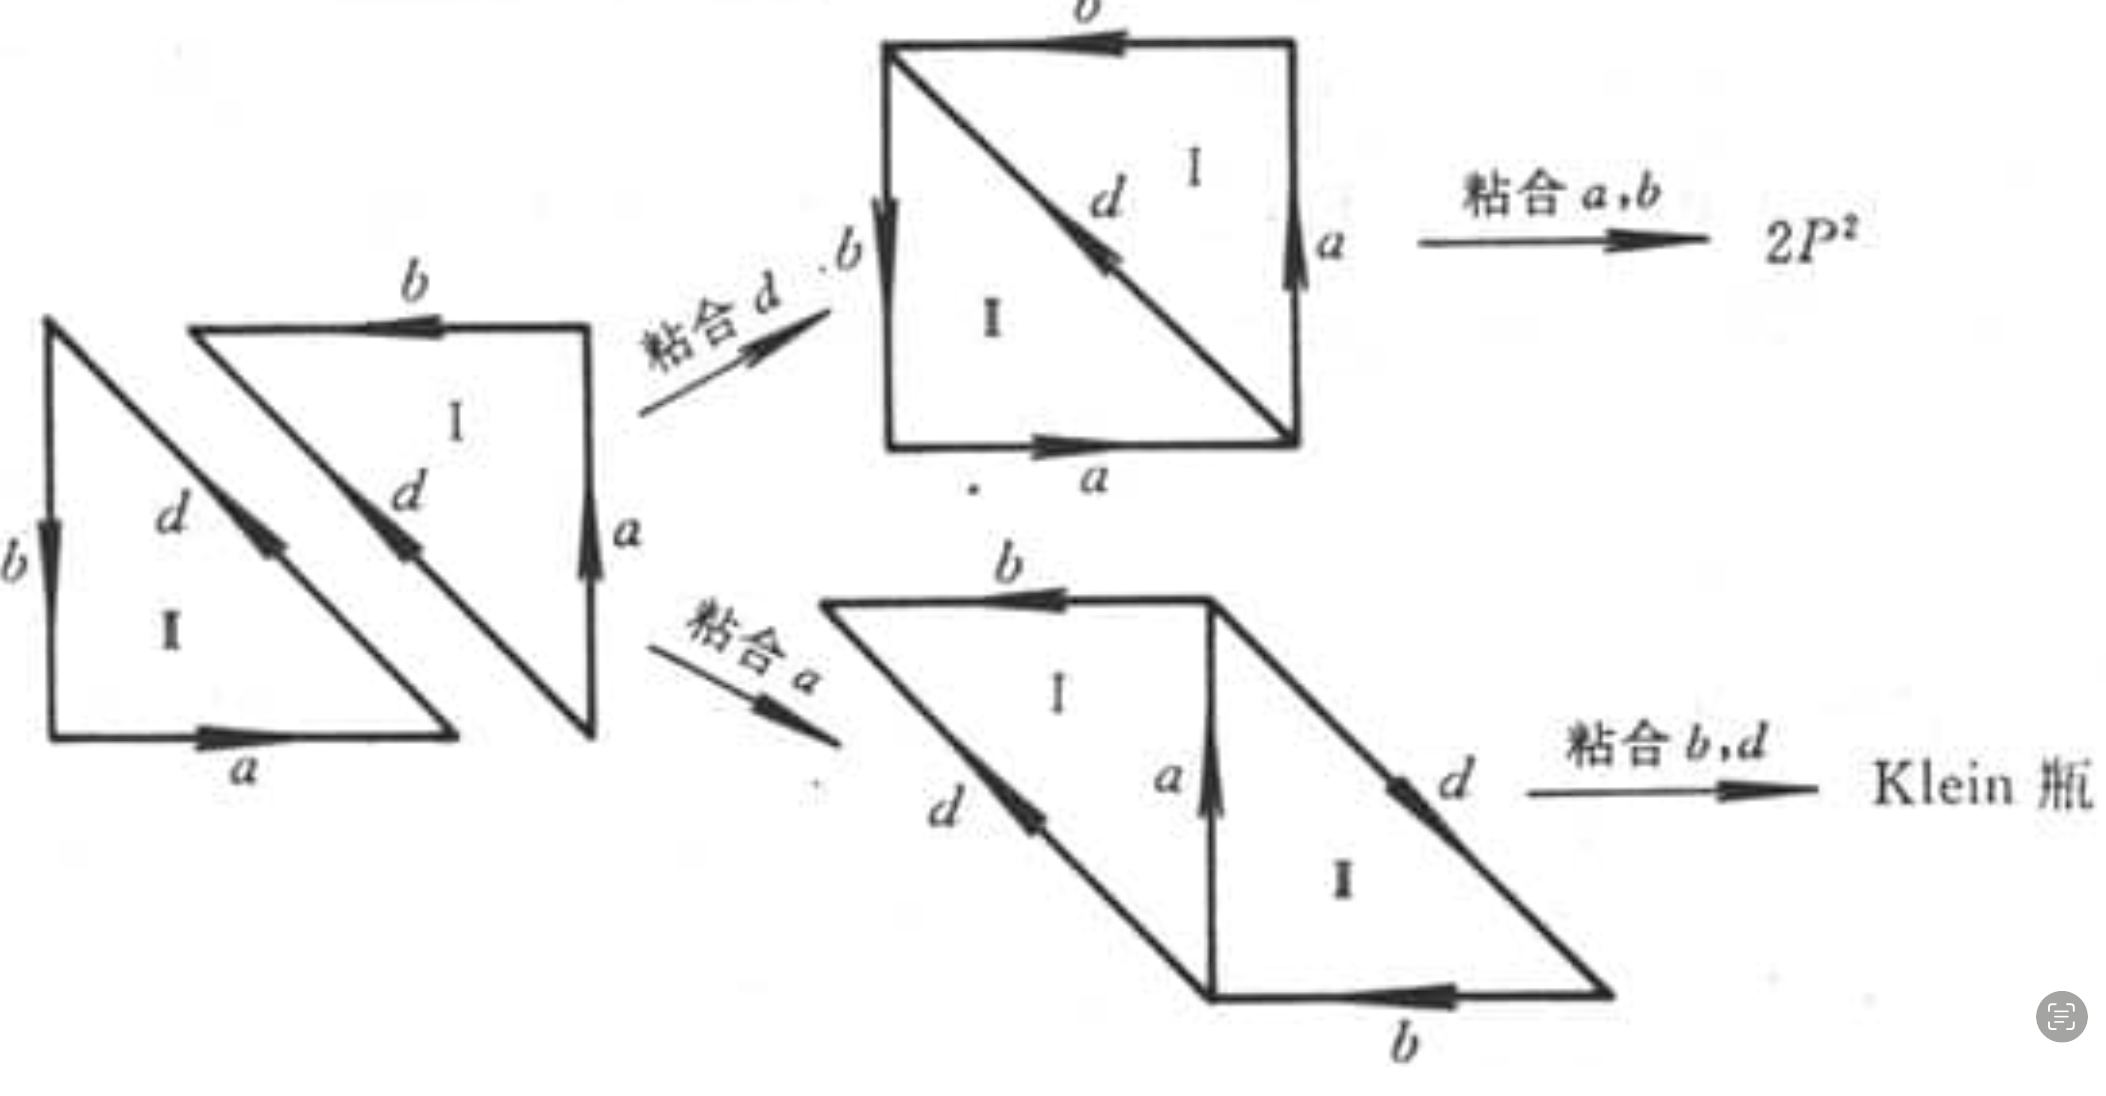
\includegraphics[width=0.4\linewidth]{image_16.png}
    \caption{}
    \label{fig:enter-label_16}
\end{figure}
\section{闭曲面分类定理}
“空间的拓扑分类(按同胚关系分类)自然是拓扑学中的一个重要问题.但是拓扑空间如此多样,不能奢望对此问题有完全的解答.即使是解决某些特定空间的分类问题的结果也是很少的.然而,闭曲面的拓扑分类问题却已得到完美的解决.闭曲面是流形中最有用的部分,它的分类定理的重要意义就更加明显了.\\
完成闭曲面分类定理的全部证明必须应用代数拓扑的结果.本章中我们用商空间方法给出它的部分证明,剩下部分放在下一章完成.”
\subsection*{闭曲面分类定理的叙述}
在上一节我们已经介绍了两大类闭曲面:可定向闭曲面\(\left\{nT^2| n\text{为非负整数} \right\} \) (n=0  时为球面) 和不可定向闭曲面\(\left\{mP^2 | m \in N \right\}\).
\begin{theorem}[闭曲面分类定理]
\(\left\{nT^2\right\}\)和\(\left\{mP^2\right\}\)不重复地列出了闭曲面的所有拓扑类型.
    则
    \begin{enumerate}
        \item 任一闭曲面或属 \(\left\{nT^2\right\}\)或属\(\left\{mP^2\right\}\) \\
        \item \(\forall n ,m \quad  nT^2 \neq mP^2\); 当\(n \neq n^{'}\)时\(nT^2 \neq n^{'}T^2\);当\(m \neq m^{'}\)时 \(m P^2 \neq m^{'} P^2\) \\
    \end{enumerate}
\end{theorem}
接下来给出计算法则 : 
\begin{figure}[H]
    \centering
    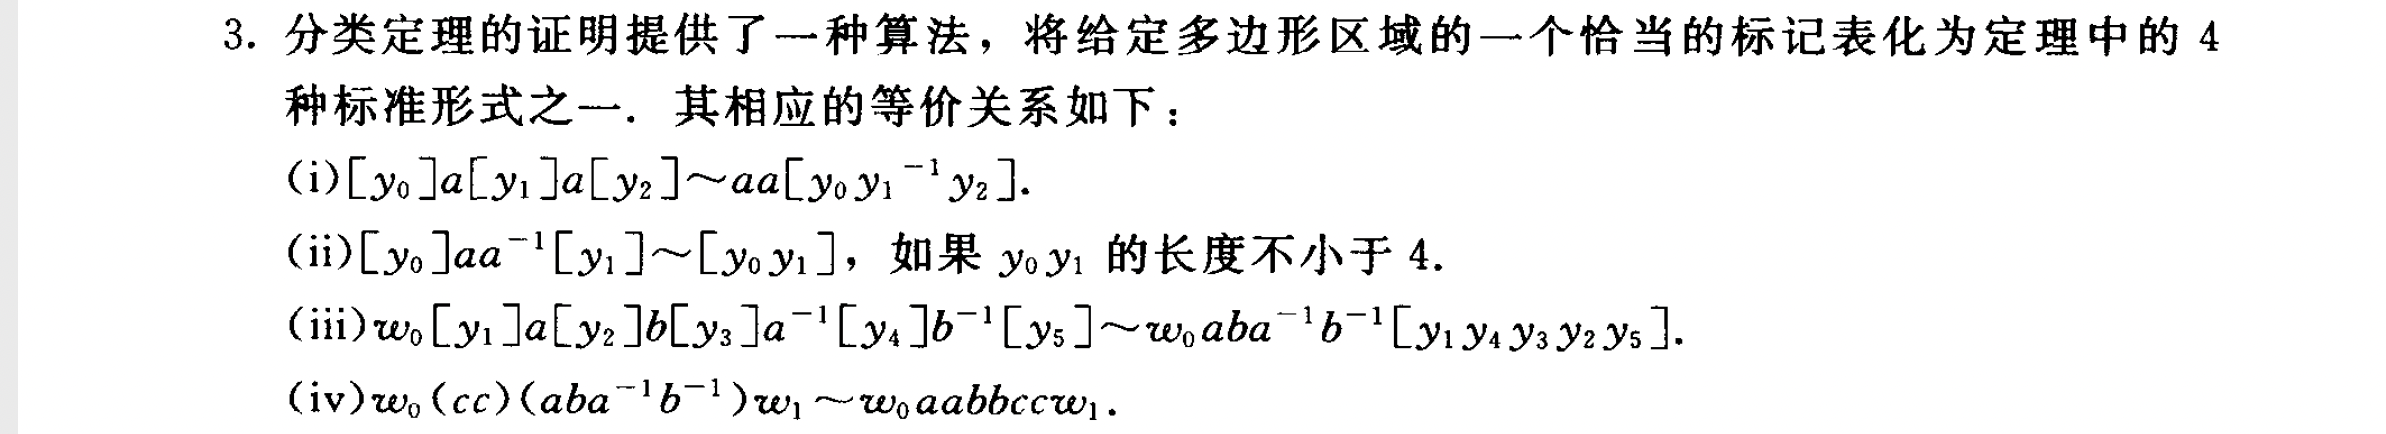
\includegraphics[width=1\linewidth]{image_17.png}
    
    
\end{figure}
